% -- Slide ---------------------------------------------------------------------
\begin{frame}{About the Tachyon Project}
    \begin{itemize}
        \item Began in summer 2010
        \item Compiler lab at UdeM
        \item Two students:
        \begin{itemize}
            \item Erick Lavoie (M.Sc.)
            \item Maxime Chevalier-Boisvert (Ph.D.)
        \end{itemize}
        \item Professor Marc Feeley
        \begin{itemize}
            \item Gambit Scheme
        \end{itemize}
        \item Professor Bruno Dufour
        \begin{itemize}
            \item Dynamic program analysis
        \end{itemize}
        \item Big project, because we like challenges
    \end{itemize}
\end{frame}
% ------------------------------------------------------------------------------

% -- Slide ---------------------------------------------------------------------
\begin{frame}{What is JavaScript?}
    \begin{itemize}
        \item JavaScript $\neq$ Java in the browser
        \item Dynamic (scripting) language
        \item Dynamic typing
        \begin{itemize}
            \item No type annotations
        \end{itemize}
        \item Basic types include:
        \begin{itemize}
            \item Doubles (no int!), strings, booleans, objects, arrays, first-class functions
        \end{itemize}
        \item Objects as hash maps
        \begin{itemize}
            \item Can add/remove properties at any time
            \item Prototype-based, no classes
        \end{itemize}
    \end{itemize}
\end{frame}
% ------------------------------------------------------------------------------

% -- Slide ---------------------------------------------------------------------
\begin{frame}{Why JavaScript?}
    \begin{itemize}
        \item JavaScript is very popular, it's everywhere
        \begin{itemize}
            \item JavaScript is the only language for web applications.
            \item Volume of JS code increasing fast, becoming more complex
        \end{itemize}

        \item Many competing implementations
        \begin{itemize}
            \item Push to move desktop apps to browsers
            \item Performance is insufficient
        \end{itemize}
        
        \item Compiling dynamic languages efficiently is challenging
        \begin{itemize}
            \item Dynamic typing, eval, etc
            \item Researchers definitely care!
        \end{itemize}
    \end{itemize}
\end{frame}
% ------------------------------------------------------------------------------

% -- Slide ---------------------------------------------------------------------
\begin{frame}{State of the Art}
    \begin{itemize}
        \item Firefox / JaegerMonkey
        \begin{itemize}
            \item Tracing JIT
            \item Compiles/specializes loop code traces
        \end{itemize}

        \item Chrome / V8
        \begin{itemize}
            \item Hidden classes
            \item Inline caches, code patching
            \item Very fast JIT compiler
            \item Very efficient GC
        \end{itemize}

        \item Is this the best we can do?
        \begin{itemize}
            \item We believe there is potential for more optimization
        \end{itemize}
    \end{itemize}
\end{frame}
% ------------------------------------------------------------------------------

% -- Slide ---------------------------------------------------------------------
\begin{frame}{Our Objectives}
    \begin{itemize}
        \item Full JavaScript (ECMAScript 5) support
        \item Retargetable JIT compiler (x86, x86-64)
        \item Meta-circularity of the VM
        \item Framework for dynamic language optimizations
        \begin{itemize}
            \item Better object representations
            \item Optimistic optimization with recompilation
            \item Fast \& efficient x86 back-end
        \end{itemize}
        \item Integration into a web-browser
        \begin{itemize}
            \item Demonstrate viability on “real” applications
        \end{itemize}
        \item Free software / OSS
    \end{itemize}
\end{frame}
% ------------------------------------------------------------------------------

% Maxime's TOC
%
% IR
% - HIR
% - IR types
% - LIR
% - IIR
%   - Annotations
%
% IR support: static definitions
% IR support: auto-generated code
% - layouts and their methods (alloc/init, accessors)
% - GC visit code
% - FFI wrappers
%
% Compilation phases
% - Present before IR?
% - Picture
%   - Parsing
%   - AST simplification/annotation
%   - AST->IR conversion
%   - IR lowering/optimization
%   - Register allocation
%   - Machine code generation
%
% Optimistic optimizations
% - Picture(s)
%
%
%

% -- Slide ---------------------------------------------------------------------
\begin{frame}{High-Level IR}
    \begin{itemize}
        \item Core JS semantics implemented in terms of primitive functions
        \begin{itemize}
            \item Act on boxed (dynamic) types
            \item Annotated for performance
                \begin{itemize}
                    \item Static linkage, force inlining, no exceptions, etc.
                \end{itemize}
        \end{itemize}

        \item Examples
        \begin{itemize}
            \item Arithmetic/comparison operators (+, -, *, /, $<$, \ldots)
            \item Property accesses (getProp, putProp, hasProp, \ldots)
        \end{itemize}

        \item Primitives implemented in terms of extended JS
    \end{itemize}
\end{frame}
% ------------------------------------------------------------------------------

% -- Slide ---------------------------------------------------------------------
\begin{frame}{JavaScript Extensions}
    \begin{itemize}
        \item JavaScript has no access to raw memory
        \begin{itemize}
            \item Essential to implement a VM/JIT
        \end{itemize}
        \item Tachyon is written in JS w/ “unsafe” extensions
        \begin{itemize}
            \item Minimizes the need to write C code (FFI)
            \item Maximizes performance
            \begin{itemize}
                \item FFIs are optimization boundaries
            \end{itemize}
        \end{itemize}
        \item JS code translated to low-level typed IR
        \begin{itemize}
            \item JS extensions: insert typed instructions in code as it is translated (Inline IR / IIR)
        \end{itemize}
    \end{itemize}
\end{frame}
% ------------------------------------------------------------------------------

% -- Slide ---------------------------------------------------------------------
\begin{frame}{Low-Level IR}
    \begin{itemize}
        \item Some similarities with LLVM
        \item SSA-based
        \item Type-annotated
        \begin{itemize}
            \item Integers, floats, booleans, raw pointers
            \item Boxed values
        \end{itemize}
        \item Low-level
        \begin{itemize}
            \item Mirrors instructions commonly found on most CPUs
            \begin{itemize}
                \item add/sub/mul/div, and/or/shift, jump/if/call, load/store, etc.
            \end{itemize}
            \item Still tries to be “machine agnostic”
            \begin{itemize}
                \item No specific endianness, no registers
            \end{itemize}
            \item Allows expressing more optimizations (specialization)
        \end{itemize}
    \end{itemize}
\end{frame}
% ------------------------------------------------------------------------------

% -- Slide ---------------------------------------------------------------------
\begin{frame}{}
\lstinputlisting{images/lt.js}
\end{frame}
% ------------------------------------------------------------------------------

% -- Slide ---------------------------------------------------------------------
\begin{frame}{}
\lstinputlisting{images/boxIsInt.js}
\end{frame}
% ------------------------------------------------------------------------------

% -- Slide ---------------------------------------------------------------------
\begin{frame}{Register Allocation}
    \begin{itemize}
        \item Linear Scan R.A. on SSA form taken from C Wimmer, M Franz 2010
        \item Combines Resolution and SSA Deconstruction
        \item Register Hints to reduce the nb of move instr.
        \item Greater granularity of lifetime intervals to reduce register pressure
        \item Parameterized register usage (blocked registers on a per-instruction basis)
        \item Block ordering preserves loop structure
        \item Main algorithm does not depend on IR
    \end{itemize}
\end{frame}
% ------------------------------------------------------------------------------

% -- Slide ---------------------------------------------------------------------
\begin{frame}{Code Generation}
    \begin{itemize}
        \item Heuristic instruction selection based on operand types (Memory Access, Immediate Value or Register Type)
        \item Parameterized function call protocol
        \item For now 
        \begin{itemize}
            \item Use the same block order as R.A.
            \item Replace string values by integers
        \end{itemize}
        \item TODO
        \begin{itemize}
            \item Working on run-time linkage of objects
        \end{itemize}
    \end{itemize}
\end{frame}
% ------------------------------------------------------------------------------

% -- Slide ---------------------------------------------------------------------
\begin{frame}{x86 Assembler}
    \begin{itemize}
        \item In-memory assembly on a “Byte” Array
        \item Jump encoding optimization based on distance to target
        \item Supports linking for static calls and jumps
        \item Text listing of generated code
        \item Supports 41/108  x86-64 general purpose instructions
        \item Support for both 32-bit and 64-bit x86
    \end{itemize}
\end{frame}
% ------------------------------------------------------------------------------

% -- Slide ---------------------------------------------------------------------
\begin{frame}{Runtime Support}
    \begin{itemize}
        \item For now
        \begin{itemize}
            \item Global object on each compiled file/unit
            \item 30-bit integer numbers only
        \end{itemize}
        \item In progress
        \begin{itemize}
            \item Object allocation code
            \item Native global object
            \item String support
        \end{itemize}
    \end{itemize}
\end{frame}
% ------------------------------------------------------------------------------

% -- Slide ---------------------------------------------------------------------
\begin{frame}{Optimistic Optimizations}
    \begin{itemize}
        \item Traditional optimizations are conservative
        \begin{itemize}
            \item Can't prove it, can't do it
            \item Dynamic languages offer little static type information
            \item Dynamic constructs problematic for analysis
            \begin{itemize}
                \item eval, load
            \end{itemize}
            \item Often can't prove validity conservatively
        \end{itemize}

        \item Optimistic optimizations
        \begin{itemize}
            \item Valid now, assume valid until proven otherwise
            \item Most dynamic programs not that dynamic
            \item Many optimizations do apply
        \end{itemize}
    \end{itemize}
\end{frame}
% ------------------------------------------------------------------------------

% -- Slide ---------------------------------------------------------------------
\begin{frame}{Example: Optimization Issues}
    \lstinputlisting{images/sum.js}
    \begin{itemize}
        \item Don't know type of \code{list} and its elements
        \begin{itemize}
            \item Dynamic type checks needed
        \end{itemize}
        \item Name \code{f} is global, can be redefined
        \begin{itemize}
            \item Fetch from global object, is-function check needed
            \item Can't trivially perform inlining
            \item \code{f} could possibly change \code{list.length}
        \end{itemize}
        \item What if we add an eval?
    \end{itemize}
\end{frame}
% ------------------------------------------------------------------------------

% -- Slide ---------------------------------------------------------------------
\begin{frame}{Realistic Assumptions}
    \begin{itemize}
        \item As programmers, it's fairly obvious to us that:
        \begin{itemize}
            \item function \code{f} is extremely unlikely to be redefined
            \item list will likely always be array of integers
        \end{itemize}

        \item Not obvious to a compiler, but, in general:
        \begin{itemize}
            \item How often are global functions redefined?
            \item How many call sites are truly polymorphic?
            \item How many function arguments can have more than one type?
            \item How often do people use eval to change local variable types?
        \end{itemize}
    \end{itemize}
\end{frame}
% ------------------------------------------------------------------------------

% -- Slide ---------------------------------------------------------------------
\begin{frame}{What Would Tachyon Do (WWTD)?}
\begin{itemize}
    \item A VM can observe the types of global variables as a program is executing
    \begin{itemize}
        \item Can assume that these types will not change
        \begin{itemize}
            \item e.g.: assume that \code{f()} will not be redefined
        \end{itemize}
        \item Compile functions with these assumptions
    \end{itemize}

    \item A VM can observe what types input arguments to a function have
    \begin{itemize}
        \item Can specialize functions based on these
        \begin{itemize}
            \item e.g.: sum(list) is always called with arrays of integers
        \end{itemize}
    \end{itemize}

    \item Types inside of function bodies can be inferred from types of globals and arguments
    \begin{itemize}
        \item Type propagation, simple dataflow analysis
    \end{itemize}
\end{itemize}
\end{frame}
% ------------------------------------------------------------------------------

% -- Slide ---------------------------------------------------------------------
\begin{frame}{Naïve JavaScript Compilation}
\begin{center}
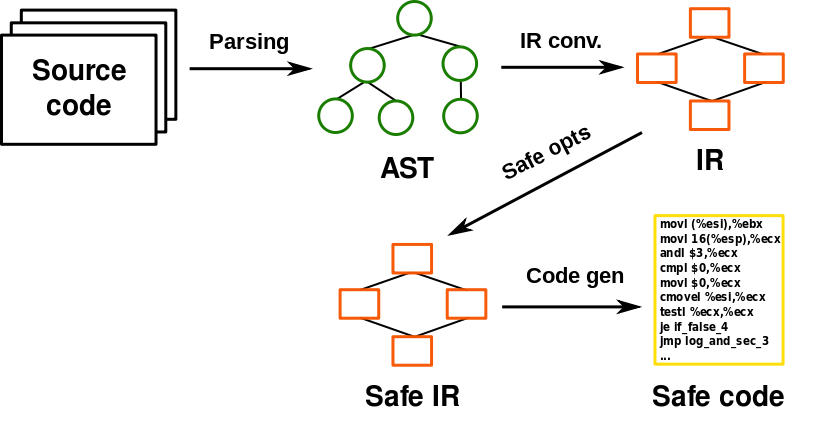
\includegraphics[width=3in]{images/transforms1}
\end{center}
\end{frame}
% ------------------------------------------------------------------------------

% -- Slide ---------------------------------------------------------------------
\begin{frame}{What Would Tachyon Do (WWTD)?}
\begin{center}
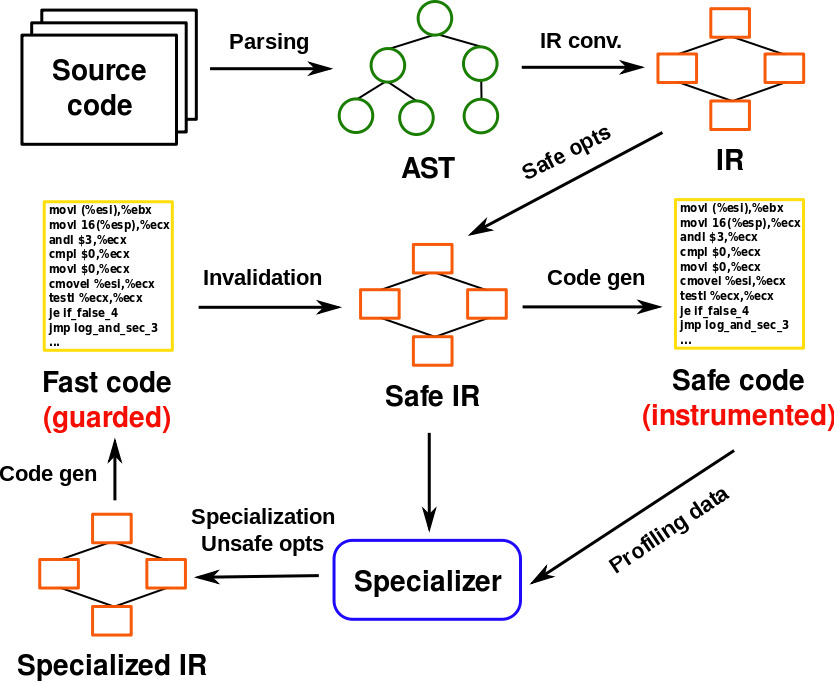
\includegraphics[width=3in]{images/transforms2}
\end{center}
\end{frame}
% ------------------------------------------------------------------------------

% -- Slide ---------------------------------------------------------------------
\begin{frame}{What Would Tachyon Do (WWTD)?}
\begin{center}
\includegraphics[height=2.8in]{images/execmodel}
\end{center}
\end{frame}
% ------------------------------------------------------------------------------

% -- Slide ---------------------------------------------------------------------
\begin{frame}{Key Ideas}
    \begin{itemize}
        \item Crucial to capture info about run time behavior
        \item Program needs to be correct at all times
        \begin{itemize}
            \item Don't need to run the same code at all times
            \item Multiple optimized versions correct at different times
        \end{itemize}

        \item Can make optimistic assumptions that may be invalidated later
        \begin{itemize}
            \item So long as we can repair our mistakes in time
            \item Code with broken assumptions must never be executed
            \item Ideally, want invalidation to be unlikely
        \end{itemize}
    \end{itemize}
\end{frame}
% ------------------------------------------------------------------------------

% -- Slide ---------------------------------------------------------------------
\begin{frame}{Type Profiling}
    \begin{itemize}
        \item Type profiling can observe:
        \begin{itemize}
            \item Frequency of calls
            \item Types of arguments to calls
            \item Types of values stored into globals
            \item Types of values stored in object fields
        \end{itemize}

        \item Goal: build fairly accurate profile of program behavior w.r.t. types
    \end{itemize}
\end{frame}
% ------------------------------------------------------------------------------

% -- Slide ---------------------------------------------------------------------
\begin{frame}{Type Propagation}
    \begin{itemize}
        \item Form of type inference
        \item Dataflow analysis
        \item Local or whole program
        \item Rules depend on language semantics, e.g.:
        \begin{itemize}
            \item add int, int $\rightarrow$ int
            \item add float, float $\rightarrow$ float
            \item mul m4x2, m2x1 $\rightarrow$ m4x1
            \item getprop o, “a” $\rightarrow$ prop\_type(o, “a”)
        \end{itemize}

        \item In the local case, inputs are function argument types, globals types, closure variable types
        \item Output: local variable types, return type
    \end{itemize}
\end{frame}
% ------------------------------------------------------------------------------

% -- Slide ---------------------------------------------------------------------
\begin{frame}{Potential Difficulties}
    \begin{itemize}
        \item Cost of profiling
        \begin{itemize}
            \item Need accurate information
        \end{itemize}
        \item Cost of recompilation
        \begin{itemize}
            \item Usage of external threads
        \end{itemize}
        \item Frequency of recompilation
        \begin{itemize}
            \item Progressive pessimization
        \end{itemize}
        \item Inherent complexity
        \begin{itemize}
            \item Find more students!
        \end{itemize}
    \end{itemize}
\end{frame}
% ------------------------------------------------------------------------------

% -- Slide ---------------------------------------------------------------------
\begin{frame}{Related Work: Type Analysis}
    \begin{itemize}
        \item M Chevalier-Boisvert, L Hendren, C Verbrugge. \textit{Optimizing
        MATLAB through just-in-time specialization}. CC 2010.
        \item F Logozzo, H Venter. \textit{RATA: Rapid Atomic Type Analysis by
        Abstract Interpretation–Application to JavaScript Optimization}. CC
        2010.
        \item S Jensen, A M\o{}ller et al. \textit{Type analysis for JavaScript}. SAS 2009.
        \item And much more\ldots
    \end{itemize}
\end{frame}
% ------------------------------------------------------------------------------

% -- Slide ---------------------------------------------------------------------
\begin{frame}{Related work: Deoptimization}
    \begin{itemize}
        \item I Pechtchanski, V Sarkar. \textit{Dynamic optimistic
            interprocedural analysis: a framework and an application}. OOPSLA 2001.
        \begin{itemize}
            \item Systematic optimistic interprocedural type analysis to optimize polymorphic call sites
        \end{itemize}
        \item Speculative inlining
        \begin{itemize}
            \item In Java, dynamic class loading can invalidate inlining decisions
            \item Implemented in Java HotSpot VM
        \end{itemize}
        \item Polymorphic inline cache
    \end{itemize}
\end{frame}
% ------------------------------------------------------------------------------

% -- Slide ---------------------------------------------------------------------
\begin{frame}{Related Work: Tracing JITs}
    \begin{itemize}
        \item HotpathVM, TraceMonkey, LuaJIT, etc.
        \item Tracing JITs are another dynamic compilation model

        \item Same basic underlying principle
        \begin{itemize}
            \item Observe program as it runs, gather data about behavior
            \item Assume current behavior will likely persist, use data to specialize program, minimize dynamic checks
        \end{itemize}

        \item Main limitations
        \begin{itemize}
            \item Local approach, detects \& examines loops
            \item Knows little about what goes on outside loops
            \item No real way of dealing with global data, optimizing object layout, etc.
        \end{itemize}
    \end{itemize}
\end{frame}
% ------------------------------------------------------------------------------

% -- Slide ---------------------------------------------------------------------
\begin{frame}{Related Work: Meta-circularity}
    \begin{itemize}
        \item JikesRVM: meta-circular Java VM
        \item Maxine VM: experimental project at Sun
        \item PyPy: Python in Python
        \begin{itemize}
            \item JIT compiler generator based on language spec.
        \end{itemize}
        \item Klein VM: Implementation of Self in Self
    \end{itemize}
\end{frame}
% ------------------------------------------------------------------------------

% -- Slide ---------------------------------------------------------------------
\begin{frame}{Distinguishing Features}
    \begin{itemize}
        \item Meta-circular with dynamic language
        \item Self-optimizing
        \item Systematic optimistic optimizations
        \item Implementation flexibility
        \begin{itemize}
            \item Function call protocol
            \item Object layout
            \item Intermediate representation
        \end{itemize}
        \item Inline IR
        \item Multithreaded compiler
    \end{itemize}
\end{frame}
% ------------------------------------------------------------------------------

% -- Slide ---------------------------------------------------------------------
\begin{frame}{Projet Status}
    \begin{itemize}
        \item ECMAScript 5 parser
        \item Translation of ASTs to SSA-based IR
        \item Simple optimizations on IR
        \begin{itemize}
            \item SCCP, value numbering, peepholes
        \end{itemize}
        \item x86 32/64 back-end with linear-scan reg. alloc.
        \item Linking of static function calls
        \item Compilation of simple programs
        \begin{itemize}
            \item Fibonacci, loops
        \end{itemize}
        \item Instruction-level statistical profiler
        \item Benchmarking framework
    \end{itemize}
\end{frame}
% ------------------------------------------------------------------------------

% -- Slide ---------------------------------------------------------------------
\begin{frame}{Projet Roadmap}
    \begin{enumerate}[1.]
        \item Bootstrap (Feb 2011)
        \begin{enumerate}[1.]
            \item Simple object representation, GC, std. lib., FFI
            \item Exceptions, closures
            \item Image loader/writer
        \end{enumerate}

        \item Competitive (June 2011)
        \begin{enumerate}[1.]
            \item Better object representation, GC, full std. lib., FFI
            \item Improved profiler, debugger
        \end{enumerate}

        \item Gravy (Dec 2011)
        \begin{enumerate}[1.]
            \item Threads 
            \item Code-patching, optimistic optimizations
            \item Browser integration
        \end{enumerate}

        \item Groovy (Post Dec. 21, 2012)
        \begin{enumerate}[1.]
            \item Persistance, contextualization
            \item On-stack replacement
        \end{enumerate}
    \end{enumerate}
\end{frame}
% ------------------------------------------------------------------------------
